\documentclass[preprint,longauthor]{aastex631}

\usepackage{blindtext}
\usepackage{amsmath}
\usepackage{subfigure}
\usepackage{graphicx}
\usepackage{listings}
\usepackage{xcolor}
\usepackage{dsfont}

\numberwithin{equation}{section}

\lstdefinestyle{pythonstyle}{
  language=Python,
  basicstyle=\ttfamily\small,
  keywordstyle=\color{blue}\bfseries,
  commentstyle=\color{teal!70!black}\itshape,
  stringstyle=\color{orange!85!black},
  numberstyle=\tiny\color{gray},
  numbers=left,
  stepnumber=1,
  numbersep=8pt,
  backgroundcolor=\color{gray!5},
  frame=tb,
  rulecolor=\color{black!30},
  breaklines=true,
  showstringspaces=false,
  tabsize=2,
  captionpos=b
}

% Note to self: Don't forget to start up Zotero when you start writing!

\begin{document}
\label{placeholder} % Delete this when done!

\title{Bayesian Inference and MCMC Methods in Astrophysics}
\author{Agastya Gaur}
\affiliation{University of Illinois at Urbana-Champaign}

\begin{abstract}
  \blindtext
\end{abstract}

\keywords{Astrophysics, Astrostatistics, Bayesian Statistics, Markov Chain Monte Carlo, Big Data}

\section{Introduction}
\label{sec:Introduction}
\subsection{The History of Astrostatistics}
In the 4th century BC, Hipparchus, attempting to estimate the length of a year, found the middle of the range of a scattered set of Babylonian solstice measurements \citep{feigelsonStatisticalChallengesModern2004}. An achievement for the time, Hipparchus's measurement marked the beginning of what would become a long-standing marriage between astronomy and statistics. In the centuries to come, a number of breakthroughs in astrostatistics followed. Notably, Tycho Brahe in the late 1500s made repeated positional measurements of stars using naked-eye observations. The data were so precise that their modeling led to Kepler's new laws of planetary motion \citep{leavesleyTychoBrahesWay2018}. Furthermore, in the 1770s, Laplace rediscovered Bayesian statistics, and over the next decade he expanded upon the theory, using it to modernize Newton's theory of gravity \citep{stiglerStudiesHistoryProbability1975}.

The biggest advance in astrostatistics before the era of computing was in 1805 when Legendre published the method of least squares regression to model the orbit of comets \citep{feigelsonStatisticalChallengesModern2004}. He theorized that the model best fit to a set of data was one that minimized the sum of the squares of the errors. Though Legendre did not provide a formal proof of the method, regarding it only as a convenient trick, later works by Robert Adrain developed formal mathematical proofs of the method \citep{merrimanHistoryMethodLeast1877}. In 1809, Gauss published his own work on least squares, using it to calculate the orbit of the dwarf planet Ceres. Controversially, he also insisted that he had discovered the method years before Legendre \citep{stiglerGaussInventionLeast1981}. Through its impact, least squares regression has cemented itself in history as one of the most important leaps in astrostatistics.

The recurring theme is clear: progress in astronomy often hinges on solving problems of statistical estimation. By the end of the century, astronomy had firmly established itself as a quantitative science, driven by the refinement of statistical methods to identify regularities in scattered measurements, fitting orbital models, and quantifying uncertainty in the presence of noise.

\subsection{The Impact of Astrophysics}

Later years brought two developments that reshaped the relationship between astronomy and statistics: the rise of physics as the foundation of astronomy and the advent of computing, which enabled unprecedented scales of data analysis. As astronomy grew increasingly intertwined with the theories of physics, the field transformed into what we now call astrophysics. Though a niche field called statistical astronomy persisted, the majority of astronomers made insufficient use of statistics in their work \citep{feigelsonStatisticalChallengesModern2004}. The focus shifted to deriving physical models from first principles, and statistical methods were often seen as secondary or even unnecessary. \citet{hubbleDistributionLuminosityElliptical1930} determined the fit for the light curve of elliptical galaxies by trial-and-error instead of regression. \citet{zwickyMassesNebulaeClusters1937} first observed dark matter using a curve fitted only by eye.

The disdain for statistics stemmed from most astrophysicists' stubborn adherence to Newtonian determinism. Physics was regarded as the fundamental law of nature and an elegant basis for astronomy, while statistics was seen as rough, approximate, and imperfect. Statistics also flourished in the social sciences, further alienating it from astrophysics.

However, statistics would not be kept away from astronomy for long. As computing machines developed, astronomers increasingly adopted new tools for both calculation and simulation. In the 1920s, one of the earliest applications appeared in the production of lunar tables. Previously, astronomers calculated the position of the Moon using complex, error-prone methods that required extensive manual computation \citep{duncombeEarlyApplicationsComputer1988}. By the 1930s, however, \citet{comrieApplicationHollerithTabulating1932} demonstrated how punch card computing machines could automate the process, making lunar ephemerides faster and more reliable. From then on to the 1970s, Comrie's work was continued by Wallace Eckert, who improved the punch-card calculations using IBM computers \citep{olleyTaskThatExceeded2018}. Like lunar calculations, galactic simulations were also performed with computational devices as early as the 1940s. \citet{holmbergClusteringTendenciesNebulae1940} modeled gravitational interactions using lightbulbs to represent galaxies, demonstrating how spiral structures could emerge. These analog demonstrations laid the groundwork for digital computer N-body simulations in the 1970s, such as \citet{toomreGalacticBridgesTails1972}, who explained tidal tails and bridges in interacting galaxies.

With these advances in computing came a natural resurgence of statistical methods in astronomy. Given the ability to automate calculations, handle larger datasets, and simulate complex systems, statistical analysis became indispensable. In the mid-20th century, the growth of galaxy surveys encouraged quantitative modeling of structure and dynamics. Early work such as \citet{lynden-bellStatisticalMechanicsViolent1967} applied statistical mechanics to stellar systems, laying the foundation for the study of galaxy formation and equilibrium. By the 1970s, statistics was increasingly recognized as a distinct methodological pillar of astronomy. \citet{peeblesStatisticalAnalysisCatalogs1973} systematically catlogued and analyzed extragalactic objects using power spectra and correlation functions, pioneering the statistical study of large-scale structure.

While the early history of the field was dominated by statistical reasoning and theory, the growth of physics and digital computation broadened this into what we now call quantitative analysis (QA). Quantitative analysis thus represents the merging of three traditions that once stood apart: the deductive rigor of physics, the inferential power of statistics, and the scalability of computation. In modern astronomy, progress often relies not on one of these strands in isolation but on their integration. QA therefore serves as both a methodological framework and a philosophy of practice, emphasizing reproducibility, uncertainty quantification, and the ability to extract physical meaning from complex data.

\subsection{The Data Deluge}

Today, astrophysics sits in a universe of complex statistical problems that demand new quantitative approaches and more computing power with each passing day. These are compounded by an unprecedented era of astronomical data generation in the 21st century. Sky surveys like Gaia DR3 alone provide astrometry and photometry for nearly two billion stars, plus more than ten million variable sources \citep{gaiacollaborationGaiaDataRelease2023}. The nineteenth data release of the Sloan Digital Sky Survey collected spectroscopic data from over 6 million objects \citep{sdsscollaborationNineteenthDataRelease2025}. Advances in CCD detectors will see data from sky surveys increase in the next decade from gigabytes to terabytes today, and possibly to petabytes in the near future. The same trend can be seen in data from NASA's Solar Dynamics Observatory, which now generates over a terabyte of data per day, and the Rubin LSST, generating close to 30 terabytes per day \citep{borneAstroinformatics21stCentury2009}. Compared to the Henry Draper Catalogue \citep{cannonHenryDraperCatalogue1918}—a century-old counterpart that cataloged roughly 200,000 stars—the explosion in data is striking.

The leap from hundreds of thousands of stars in the Henry Draper Catalogue to billions in Gaia represents more than a change in scale: it is a qualitative transformation in what science becomes possible. With the Draper Catalogue, astronomers could classify stellar spectra and trace broad patterns in stellar populations. With Gaia, it is now possible to reconstruct the full three-dimensional structure and kinematics of the Milky Way, identify hypervelocity stars, and test theories of Galactic evolution with unprecedented detail. Where older surveys allowed the identification of a few rare stellar types, modern surveys allow systematic searches for extreme outliers across billions of objects, transforming the statistical character of astronomy.

This data deluge makes QA indispensable. Large-scale surveys now span the entire electromagnetic spectrum, from radio (e.g., LOFAR, ALMA) to X-ray and gamma-ray observatories such as Chandra and Fermi. Multi-messenger astronomy adds yet another layer, with gravitational waves detected by LIGO/Virgo and high-energy neutrinos from IceCube \citep{abbasiSearchIceCubeSubTeV2023}. Time-domain surveys such as ZTF and the upcoming LSST produce streams of transient and variable sources, producing large data volumes and data rates. Each dataset has distinct noise properties, resolutions, and systematic biases, making multi-wavelength integration a formidable statistical task. The ability to extract meaningful insights from these massive datasets is crucial for advancing our understanding of the universe.

\subsection{Statistical Challenges in Modern Astrophysics}

Two recurring types of statistical challenges emerge across astrophysics. The first challenge is that noisy, incomplete, and often degenerate data have uncertain theoretical statistical distributions. In addition, the number, complexity, and degeneracy of physical parameters poses major challenges \citep{schaferFrameworkStatisticalInference2015}. For example, in exoplanet studies, radial velocity measurements can only determine a planet’s minimum mass because they do not contain orbital inclination \citep{lovisRadialVelocityTechniques2010}. In cosmology, measurements of the cosmic microwave background couple the effects of the Hubble constant, the amount of ordinary matter, and dark energy, so isolating any one factor requires prior assumptions about the others \citep{christensenParameterEstimationGravitational2022}. Even within galaxies, rotation curve studies must weight the balance between visible stars and invisible dark matter. Each of these cases requires careful statistical treatment to avoid misleading conclusions.

The second challenge is that the large volume of data and model complexity creates equally daunting problems of computing time and power. As noted above, the Rubin Observatory LSST will generate tens of terabytes of imaging data per night \citep{borneAstroinformatics21stCentury2009}, while Gaia has already released petabyte-scale catalogs \citep{gaiacollaborationGaiaDataRelease2023}. Brute-force exploration of parameter spaces is simply impossible at these scales. Efficient algorithms and scalable statistical methods are required to render analysis computationally tractable \citep{huijseComputationalIntelligenceChallenges2014}. Together, these issues create a need for QA frameworks that can handle degeneracy in complex parameter spaces, model complexities, and scale efficiently with massive datasets.

\subsection{Bayesian Inference and MCMC in Context}

In this domain, Bayesian inference via Markov Chain Monte Carlo (MCMC) methods naturally emerges as a potential solution. Bayesian inference offers a principled framework for parameter estimation in complex systems. MCMC methods provide an effective way to explore parameter spaces by sampling from posterior distributions. This has become one of the most widely used and versatile approaches \citep{vontoussaintBayesianInferencePhysics2011}. Computational models are becoming far more complex, and the data being analyzed is often noisy and incomplete. Bayesian methods, with their ability to incorporate prior parameter constraints and handle uncertainty, are particularly well-suited to these challenges. MCMC methods, in particular, provide a practical way to sample from complex posterior distributions that arise in Bayesian analysis. This makes them invaluable for parameter estimation, model comparison, and uncertainty quantification.

%Flesh out this paragraph more
Another reason for the appeal of Bayesian methods is their contrast with frequentist approaches. Frequentist methods, which were dominant through much of the 20th century, emphasize point parameter estimates and confidence intervals derived from repeated sampling arguments \citep{trottaBayesSkyBayesian2008}. Bayesian inference, in contrast, provides full posterior probability distributions for parameters, naturally incorporating prior information from physics or earlier observations. This framework is particularly powerful where data are sparse, noisy, and incomplete.

The wider adoption of Bayesian statistics in astronomy gained momentum in the late 20th century. Cosmologists have applied Bayesian methods to the cosmic microwave background to extract cosmological parameters from noisy sky maps \citep{tegmarkKarhunenLoeveEigenvalueProblems1997}. In exoplanet science, Bayesian inference became common in the 1990s and 2000s for modeling radial velocity curves and transit signals in the era of larger and more precise datasets \citep{gregoryBayesianAnalysisExtrasolar2005}. Pulsar timing, supernova cosmology, and gravitational lens modeling similarly saw wider use of Bayesian methods. The trend reflects a broader recognition that many of astronomy’s hardest problems demand not just point estimates, but principled uncertainty quantification.

We review here Bayesian inference and MCMC within an astrophysical perspective because of their flexibility, principled uncertainty quantification, and growing ubiquity across astrophysics. In \hyperref[sec:Methodology]{Section II}, the methodology section develops a working foundation: here we review Bayesian statistics, priors, and likelihood construction in realistic astronomical settings. We cover toy examples before escalating to domain-relevant formulations. Then, we introduce Monte Carlo methods and build to Markov Chain Monte Carlo, deriving the Metropolis family and related samplers, providing step-by-step Python implementations on simple problems.

\hyperref[sec:CaseStudies]{Section III} presents three focused case studies that illustrate how Bayesian–MCMC pipelines advance frontiers in different subfields. For exoplanet direct detection, the section outlines the observational context and the central challenge of disentangling planetary signals from stellar activity and disk structure in direct imaging. It then outlines joint stellar–planet modeling with Gaussian processes and Bayesian classification frameworks for robust detections and non-detections, highlighting benefits and failure modes in low SNR regimes. For CMB parameter estimation, we consider geometric degeneracies in the power spectrum and shows how MCMC accelerators and parallelizable frameworks enable efficient exploration and evidence calculations, including tradeoffs between sampler sophistication and wall-clock efficiency. For gravitational-wave inference, we consider waveform fitting in high-dimensional parameter spaces, discuss the cost of likelihood evaluations, and motivate gradient-informed MCMC strategies that reduce computation without compromising accuracy.

Finally, in \hyperref[placeholder]{Section IV} and \hyperref[placeholder]{V} we compare cases where Bayesian–MCMC excels with those where complementary methods are more appropriate, identify methodological gaps revealed by the case studies, and outline opportunities for future work in astrophysics and related fields that face similar statistical and computational challenges.

\section{Methodology}
\label{sec:Methodology}

\subsection{Bayesian Preliminaries} % You can also talk about the difference between Bayesian and Frequentist Stats here
The aim of Bayesian statistics is simple: determine $P(H|D)$, or the probability of a hypotheses $H$ being true given data $D$. A hypothesis is any statement that can be true or false, and data is any information that can be used to evaluate the hypothesis. For example, imagine rolling a die. A hypothesis $H$ would that the die roll is a 3. The data $D$ is the result of the die roll.

Hypotheses live in the \textit{hypothesis space}, which is the set of all possible hypotheses of a system \citep{brewer1BayesianInference2018}. Going back to the die example, the hypothesis space is $\{1,2,3,4,5,6\}$. The hypothesis space will also have a probability distribution, or a \textit{prior}, written as $P(H)$. The prior is the probability of each hypothesis being true before seeing any data. For a fair die, the prior is uniform. It's $\frac{1}{6}$ for all $H$ in the hypothesis space. In other words, $P(H)$ is the probability of the hypothesis being true.

The data $D$ also has a probability distribution called the \textit{evidence}, $P(D)$ \citep{brewer1BayesianInference2018}. The evidence is the probability of seeing the data before knowing anything about the hypothesis. In the die example, if you roll a 3, then $P(D)$ is $\frac{1}{6}$ because there is a $\frac{1}{6}$ chance of rolling a 3 on a fair die. The evidence lives in the \textit{data space}, which is the set of all possible data of a system. In the die example, the data space is also $\{1,2,3,4,5,6\}$.

A \textit{likelihood}, $P(D|H)$, is the probability of seeing the data assuming that the hypothesis is true. In the die example, if $H$ is that the die roll is a 3, then $P(D|H)$ is 1 if the die roll is a 3 and 0 otherwise. Using the prior, evidence, and likelihood to calculate $P(H|D)$, which is the probability of a hypothesis being true given the data. This is called the \textit{posterior}. In the die example, if you roll a 3, then $P(H|D)$ is 1 if $H$ is that the die roll is a 3 and 0 otherwise.

The framework for finding $P(H|D)$ is called Bayes' Theorem, and it forms the center of Bayesian inference. It can be derived using two rules \citep{coxProbabilityFrequencyReasonable1946}. Firstly, the probability that a hypothesis is true and the probability that it is not true add up to 1:

\begin{equation}
  P(H) + P(\tilde{H}) = 1.
\end{equation}

The second rule is the product rule, which states:

\begin{equation}
  P(H)P(D|H) = P(D)P(H|D).
\end{equation}

This can be trivially rearranged to give Bayes' Theorem:

\begin{equation}
  \label{eq:bayes_theorem}
  P(H|D) = \frac{P(H)P(D|H)}{P(D)}.
\end{equation}

In other words, given the prior, evidence, and the likelihood, you can calculate the posterior $P(H|D)$.

\subsubsection{Example: The Double-Headed Coin}
The previous example of a die roll was trivial. The data, the result of the die roll, completely determined the hypothesis. Bayesian statistics becomes more useful when the data is incomplete, as is often the case in Astrophysics.

To demonstrate this, consider the following setup. You have 5 coins, four of which are fair, and one of which is double-headed. You pick a coin at random and flip it, and it lands heads. \textit{What is the probability that you picked the double-headed coin?}

The first step is to determine $H$ and $D$ from the hypotheses and data spaces. The hypothesis space is $\{\text{Picked Fair},\text{Picked Double-Headed}\}$. For the sake of conciseness, it can be written as $\{\text{fair},\text{double}\}$. For this problem, we hypothesize that the double-headed coin was picked. So, $H$ is 'double'. The data space is $\{\text{heads},\text{tails}\}$, and for this problem, $D$ is 'heads'.

Next, we determine the prior and evidence. There are 4 fair coins and 1 double-headed coin, so it is easy to find for the prior that $P(\text{fair}) = \frac{4}{5} = 0.8$ and $P(\text{double}) = \frac{1}{5} = 0.2$. The evidence is more complex to find in this case. Since the chance of flipping heads or tails includes the case that you picked up the double headed coin, the evidence cannot simply be 50-50. We must calculate the probability of getting heads and tails across all the coins:

\begin{align*}
  P(\text{heads}) &= \frac{4(0.5)+1(1)}{5} = 0.6 \\
  P(\text{tails}) &= \frac{4(0.5)+1(0)}{5} = 0.4
\end{align*}

Note the implicit rule for any space:

\begin{equation}
  \sum_n P(x_n) = 1,
\end{equation}

where $x_n$ is a value in a space.

The final step before solving is to find the likelihood, $P(\text{heads}|\text{double})$. This is trivially 1, as you can only get heads from the double-headed coin. Now, we can solve for the posterior:

\begin{align*}
  P(\text{double}|\text{heads}) &= \frac{P(\text{double})P(\text{heads}|\text{double})}{P(\text{heads})} = \frac{0.2}{0.6} = \boxed{0.\bar{3}}
\end{align*}

Before incorporating the data, the probability of picking the double headed coin was $0.2$, but by using Bayesian statistics, we were able to "learn" from the data and increase the probability to $0.\bar{3}$. This is a simple example, but it demonstrates the power of Bayesian statistics in the face of incomplete data.

\subsection{Bayesian Statistics in Astrophysics}

In an astrophysical context, Bayes' Theorem is used to calculate the probability of \textit{parameters}, $\theta$, of a model rather than a hypothesis \citep{brewer1BayesianInference2018}.

\begin{equation}
  \label{eq:bayes_theorem_params}
  P(\theta|D) = \frac{P(\theta)P(D|\theta)}{P(D)}.
\end{equation}

Take, for example, measurements of the radial velocity of a star over time. When a start hosts an orbiting planet, both bodies orbit a common center of mass. This induces a 'wobble' in the star's motion which is detected as periodic Doppler shifts from the star's spectrum, also known as the \textit{radial velocity}. The radial velocity $v_r(t)$ of a star with a single planet in a strictly circular orbit can be modeled by the following equation:

\begin{equation}
  \label{eq:rv_model}
  v_r(t) = K \sin\left(\frac{2\pi t}{T} + \phi\right),
\end{equation}

where $K$ is the velocity semi-amplitude, $T$ is the orbital period, and $\phi$ is a phase offset. Thus, the parameters of this model are $\theta = \{K,P,\phi\}$. This is a simplified model derived from \citet{lovisRadialVelocityTechniques2010}. Some parameters, such as eccentricity, system velocity, and argument of periapsis, have been omitted for simplicity.

One could measure the radial velocity of a star over a certain time period and obtain the data shown in \autoref{fig:rv_data}.

\begin{figure}[ht!]
\centering
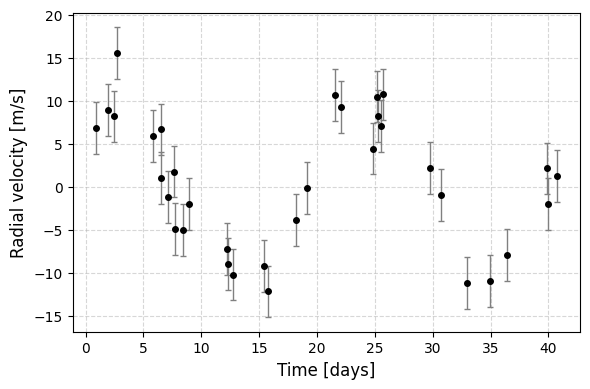
\includegraphics[width=0.7\textwidth]{../scripts/2.2/figures/data.png}
\caption{Simulated radial velocity data of a star with a single orbiting planet. Each point has an error of three standard deviations. The data is noisy and incomplete, making it difficult to determine the parameters of the model.}
\label{fig:rv_data}
\end{figure}

Bayes' Theorem can be used to determine the posterior distribution of the parameters using the noicy, incomplete data. In this case, \autoref{eq:bayes_theorem} becomes:

\begin{equation}
  P(K,T,\phi|D) = \frac{P(K,T,\phi)P(D|K,T,\phi)}{P(D)}.
\end{equation}

To start, we must determine the prior, $P(K,T,\phi)$. For simplicity, we can assume that the parameters are independent, so the prior can be written as:

\begin{equation}
  P(K,T,\phi) = P(K)P(T)P(\phi).
\end{equation}

Since we know nothing about the priors, it is reasonable to assume that they are uniformly distributed in a certain range. Looking at the data, we can see that the velocity semi-amplitude $K$ is between 5 and 15 m/s, the period $T$ is between 20 and 30 days, and the phase offset $\phi$ is between 0 and $2\pi$. Thus, the priors are:

\begin{equation*}
  P(K) = \begin{cases}
    \frac{1}{10} & 5 < K < 15 \\
    0 & \text{otherwise}
  \end{cases} \qquad
  P(T) = \begin{cases}
    \frac{1}{10} & 20 < T < 30 \\
    0 & \text{otherwise}
  \end{cases} \qquad
  P(\phi) = \begin{cases}
    \frac{1}{2\pi} & 0 < \phi < 2\pi \\
    0 & \text{otherwise}
  \end{cases}
\end{equation*}

and the combined prior is then:

\begin{equation}
  P(K,T,\phi) = \begin{cases}
    \frac{1}{200\pi} & 5 < K < 15, 20 < T < 30, 0 < \phi < 2\pi \\
    0 & \text{otherwise}
  \end{cases}
\end{equation}

Next, we must determine the likelihood, $P(D|K,T,\phi)$, or the probability of seeing the data given the parameters. To do this, we calculate the probability of seeing each data point given what the model would predict for that data point. We can assume the model prediction is the mean of a normal distribution of possible points, and the error of each data point is the standard deviation. Using this, we can calculate the probability of obtaining a data point $d_i$ at time $t_i$. Multiplying the probabilities of all the data points gives the probability of seeing the full dataset, which is the likelihood. Mathematically, this is:

\begin{equation}
  P(D|K,T,\phi) = \prod_{i=1}^{N} \frac{1}{\sqrt{2\pi\sigma_i^2}} \exp\left(-\frac{(D_i - v_r(t_i;K,T,\phi))^2}{2\sigma_i^2}\right),
\end{equation}

Substituting values for each parameter gives the likelihood of seeing the data given the parameters.

Finally, we must determine the evidence, $P(D)$. It's obvious that when integrating the posterior over the entire parameter space, it must equal one, as the parameters are certain to take on some value within the space. Thus, the evidence can be found by rearranging the equation:

\begin{align}
  1 &= \iiint P(K,T,\phi|D) dK dT d\phi\nonumber \\
  1 &= \iiint \frac{P(K,T,\phi)P(D|K,T,\phi)}{P(D)} dK dT d\phi \nonumber \\
  \therefore P(D) &= \iiint P(K,T,\phi)P(D|K,T,\phi) dK dT d\phi
\end{align}

Note that this integral is analytically intractable, so it must be calculated numerically.

Using the data in \autoref{fig:rv_data}, we can calculate the posterior distribution of the parameters using the code given in \autoref{appx:A}. Note that the code uses the log-prior and log-likelihood. These are used to prevent any underflow errors in the program. These can be calculated by taking the natural logarithm of the prior and likelihood, respectively. The posterior can then be calculated by adding the log-prior and log-likelihood, and then exponentiating the result, then normalizing with the evidence.

\begin{equation}
  P(K,T,\phi|D) = \frac{e^{\log(P(K,T,\phi)) + \log(P(D|K,T,\phi))}}{P(D)}
\end{equation}

The program evaluates the posterior on a grid of 100 points for each parameter, giving a total of $100^3 = 1,000,000$ points. The posterior is also cumulatively summed at every evaluated point, giving a numerical estimate of the evidence for normalization. Finally, the marginal posteriors of each parameter are calculated from the total posterior by integrating over the other two parameters:
\begin{align}
  P(K|D) &= \iint P(K,T,\phi|D) dT d\phi \\
  P(T|D) &= \iint P(K,T,\phi|D) dK d\phi \\
  P(\phi|D) &= \iint P(K,T,\phi|D) dK dT
\end{align}
The results of the code are shown in \autoref{fig:bf_posteriors}.

\begin{figure}[ht!]
\centering

\subfigure[$\mu = 9.99$ m/s $\quad \sigma = 0.73$ m/s]{%
    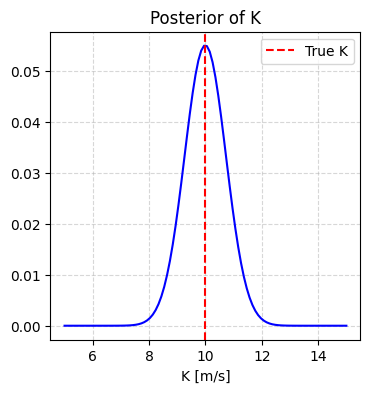
\includegraphics[width=0.32\textwidth]{../scripts/2.2/figures/k-posterior.png}%
    \label{fig:k_posterior}%
}
\hfill
\subfigure[$\mu = 21.72$ days $\quad \sigma = 0.44$ days]{%
    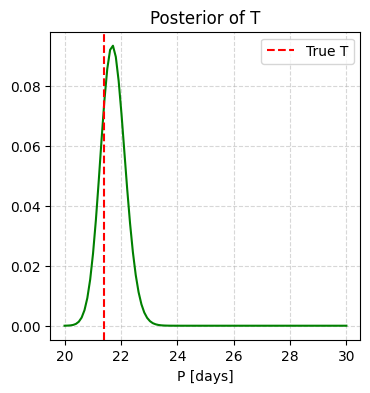
\includegraphics[width=0.32\textwidth]{../scripts/2.2/figures/t-posterior.png}%
    \label{fig:t_posterior}%
}
\hfill
\subfigure[$\mu = 0.89$ rad $\quad \sigma = 0.13$ rad]{%
    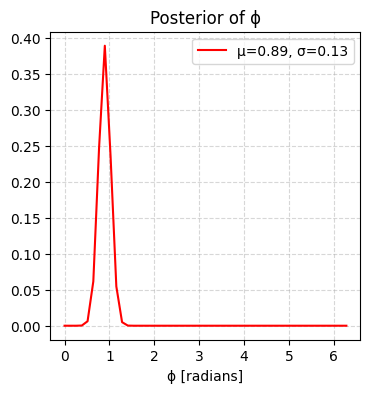
\includegraphics[width=0.32\textwidth]{../scripts/2.2/figures/phi-posterior.png}%
    \label{fig:phi_posterior}%
}
\caption{The marginal posterior distributions of the parameters $K$, $T$, and $\phi$ given the data in \autoref{fig:rv_data}. These posteriors are normalized with a numerically calculated evidence.}
\label{fig:bf_posteriors}
\end{figure}

In reality, we will never know the exact parameters of a system, but posterior distributions give us a close estimate. To quantify how close the estimate is, we will compare the posterior distributions to the true parameters, which are $K=10$ m/s, $T=25$ days, and $\phi=\frac{\pi}{4}$. It is clear to see that the true values are within one standard deviation of the mean of each posterior distribution, indicating that the Bayesian method was successful in estimating the parameters.

\begin{figure}[ht!]
\centering
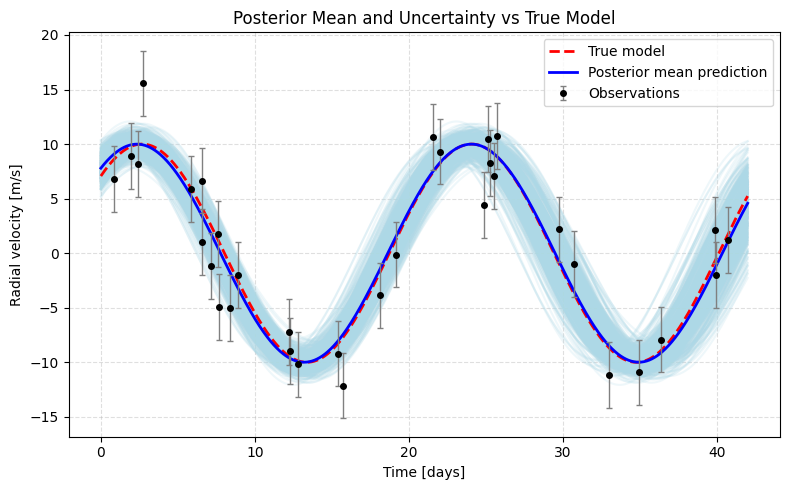
\includegraphics[width=0.7\textwidth]{../scripts/2.2/figures/prediction.png}
\caption{The radial velocity data from \autoref{fig:rv_data} along with the mean prediction from the posterior distributions in \autoref{fig:bf_posteriors}. The shaded region represents one standard deviation from the mean prediction.}
\label{fig:prediction}
\end{figure}

\autoref{fig:prediction} shows the true model along with the mean prediction from the posterior distributions. Thus, we can apply Bayes' Theorem to predict the parameters for astrophysical models. However, this method is computationally expensive. Computing this numerically, we would have to iterate through all combinations of all values of each parameter. With $n$ parameters and $m$ possible values for each parameter, this algorithm would have a time complexity of $O(m^n)$, which is infeasible for even small $n$ and $m$. To solve this problem, we can use \textit{Monte Carlo methods}.

\subsection{Monte Carlo Sampling}
The primary computational challenge in brute force Bayesian inference arises from evaluating the posterior probability at every point in the parameter space. One way to reduce this cost is to sample only a subset of points, distributed according to the posterior itself. These points are called \textit{draws}. If, by some method, a set of draws were obtained, it would be possible to calculate expectation values from the explicit posterior using only the sampled points \citep{vontoussaintBayesianInferencePhysics2011}. This is the idea behind \textit{Monte Carlo Sampling}, which can be used to approximate integrals and expectations that would otherwise require explicit evaluation over a continuous space.

If we know a probability density explicitly, the expectation value of some variable $x$ can be calculated as:

\begin{equation}
  \langle x \rangle = \int x P(\theta) dx.
\end{equation}

Using a set of $N$ values of $x$ drawn using Monte Carlo, this can be approximated as:

\begin{equation}
  \langle x \rangle \approx \frac{1}{N} \sum_{i=1}^{N} x_i,
\end{equation}
which generalizes naturally to higher-dimensional parameter spaces, though convergence can become slower as dimensionality increases.

$x$ is a function of the parameters, and can be defined arbitrarily to calculate the expectation value of any value of interest. Given a probability density $P(\theta_1,\theta_2,\hdots,\theta_n)$, some forms of $x$ are listed in \autoref{tab:x_forms}.
\begin{deluxetable}{ll}
  \tablewidth{0pt}
  \tablenum{1}
  \tablehead{
    \colhead{$x$} & \colhead{Description}
  }
  \startdata
    $\theta_i$ & Expectation value of parameter $\theta_i$ \\
    $\theta_i^2$ & Variance of parameter $\theta_i$ \\
    $f(\theta_1,\theta_2,\hdots,\theta_n)$ & Expectation value of any function of the parameters \\
    $\mathds{1}(\theta_i = a)$ & Probability that $\theta_i = a$ \\
    $\mathds{1}(a \le \theta_i \le b)$ & Probability that $\theta_i$ is in the range $[a,b]$ \\
    $\mathds{1}(\text{condition})$ & Probability that the condition is true \\
  \enddata
  \caption{Forms of $x$ to calculate expectation values of different quantities.}
  \label{tab:x_forms}
\end{deluxetable}

The usefulness of Monte Carlo sampling becomes apparent when we revisit the computation of marginal posteriors. In the previous example, we used the posterior to calculate the marginal posteriors of each parameter. In the brute force method, this was found by integrating the posterior over all other parameters. Monte Carlo makes this simpler. If we have a set of $N$ draws from the posterior of a parameter space with parameters, $\{\theta_1,\theta_2,\hdots,\theta_n\}$, we can obtain draws for a certain parameter $\theta_i$ by simply ignoring all other parameters. A simple histogram of the draws of $\theta_i$ then gives the marginal posterior of $\theta_i$. This is much simpler than integrating over all other parameters, especially in high-dimensional parameter spaces.

\subsection{Markov Chain Monte Carlo}
Before we can use Monte Carlo sampling, we must first obtain draws from the posterior. \textit{Markov Chain Monte Carlo} (MCMC) is one of the many methods used to obtain these draws, and in modern astrophysics, has become a standard tool for Bayesian inference. Using MCMC, the posterior of even a high-dimensional parameter space can be numerically mapped without using unfeasible amounts of computing power \citep{trottaBayesSkyBayesian2008}. MCMC does this by creating a sequence of draws in the form of a \textit{Markov Chain}.

\subsubsection{Markov Chains}

A Markov Chain is a sequence of random variables, $x_0, x_1, \hdots, x_n$, where the probability of each variable only depends on the previous variable. This is known as the \textit{Markov Property}, and can be written mathematically as:

\begin{equation}
  P(x_{n+1}|x_n,x_{n-1},\hdots,x_0) = P(x_{n+1}|x_n).
\end{equation}

To create a Markov chain, we must first decide an initial value $x_0$ using an initial probability distribution $P_0(x_0)$. After this, the probability distribution of the next value is evolved from the previous probability distribution using a \textit{transition probability} $T_n(x_n,x_{n+1})$. The next value is then drawn using the new probability density.

\begin{equation}
  P(x_{n+1}) = P(x_n)T_n(x_n,x_{n+1})
\end{equation}
This process can be repeated as many times as necessary.

If the transition probability does not depend on the point in the chain, the chain is \textit{homogenous}, or \textit{stationary}. We can then write the transition probability as $T(x_n,x_{n+1})$ \citep{neal1993probabilistic}.

Markov chains can be shown to converge to a \textit{stationary distribution} $P^*(x)$, which is independent of the initial distribution \citep{trottaBayesSkyBayesian2008}. A stationary distribution, once reached, does not change as the chain evolves further.

Markov chains can also be \textit{ergodic}, which means that a stationary distribution can be reached from any initial distribution. A chain being ergodic also implies its irreducibility and aperiodicity \citep{neal1993probabilistic}. Irreducibility means that it is possible to reach any point in the space from any other point, and aperiodicity means that the chain does not get stuck in cycles \citep{vontoussaintBayesianInferencePhysics2011}.

In the context of Bayesian inference, the goal of MCMC is to construct a Markov chain whose stationary distribution is the unknown posterior distribution. To ensure that the chain converges to the desired posterior, the choice of transition probability $T(x_n, x_{n+1})$ is crucial. The transition rule must satisfy the condition of \textit{detailed balance}, which guarantees that, at equilibrium, the probability flow between any two states is symmetric:
\begin{equation}
  P(x_n)T(x_n, x_{n+1}) = P(x_{n+1})T(x_{n+1}, x_n).
\end{equation}
This condition ensures that the chain does not drift away from the target distribution once it has been reached \citep{vontoussaintBayesianInferencePhysics2011}.

\subsubsection{The Metropolis-Hastings Algorithm}

One of the simplest and most widely used algorithms that satisfies detailed balance is the \textit{Metropolis algorithm} \citep{metropolisEquationStateCalculations1953}. More specifically, its generalization, the \textit{Metropolis–Hastings algorithm} \citep{hastingsMonteCarloSampling1970}. The algorithm constructs a Markov chain by iteratively proposing new states in the parameter space and deciding whether to accept or reject them based on the target distribution. \citet{brewer1BayesianInference2018} outlines the steps of the Metropolis-Hastings algorithm as follows:

\begin{enumerate}
  \item Initialize the chain with a starting point $x_0$.
  \item Generate a candidate point $x_{n+1}$ from a proposal distribution $q(x_{n+1}|x_n)$ based on the current state $x_n$.
  \item Accept or reject the proposal
  \item Repeat steps 2 and 3 for a large number of iterations to generate a sequence of samples.
\end{enumerate}

The algorithm depends on two things: the proposal distribution $q(x_{n+1}|x_n)$ and the acceptance criterion. Commonly, a 'random walk' proposal is used to generate candidates by adding a small random perturbation to the current state. For an $n$-dimensional parameter space, the random walk proposal is a symmetric (usually Gaussian) distribution, also of $n$-dimensions, with the current state as its mean \citep{vontoussaintBayesianInferencePhysics2011}. If the proposal distribution is indeed symmetric, then the following is implied:
\begin{equation}
  \label{eq:symmetric_proposal}
  q(x_{n+1}|x_n) = q(x_n|x_{n+1}).
\end{equation}
In this case, the Metropolis-Hastings algorithm simplifies to the original Metropolis algorithm \citep{brewer1BayesianInference2018}. Asymmetric proposal distributions are more general, and can also be used. However, they are less common in practice.

The acceptance criterion is based on the ratio of the posterior at the proposed and current states, adjusted by the proposal distribution. This is the probability of the proposal being accepted. Mathematically, this is:

\begin{equation}
  \alpha = \min\left(1, \frac{P(x_{n+1}|D) q(x_n|x_{n+1})}{P(x_n|D) q(x_{n+1}|x_n)}\right) = \min\left(1, \frac{P(D|x_{n+1}) P(x_{n+1}) q(x_n|x_{n+1})}{P(D|x_n) P(x_n) q(x_{n+1}|x_n)}\right).
\end{equation}
If the proposal distribution is symmetric, we can further apply \autoref{eq:symmetric_proposal} to get:
\begin{equation}
  \alpha = \min\left(1, \frac{P(D|x_{n+1}) P(x_{n+1})}{P(D|x_n) P(x_n)}\right).
\end{equation}
Working with log-priors and log-likelihoods makes this even simpler:
\begin{equation}
  \log(\alpha) = \min\left(0, \log(P(D|x_{n+1})) + \log(P(x_{n+1})) - \log(P(D|x_n)) - \log(P(x_n))\right).
\end{equation}

This criterion accepts any proposal that increases the posterior probability, while proposals that decrease it are accepted with a probability proportional to the decrease. If a proposal is rejected, the current state is counted again. This allows the chain sample high-probability regions more frequently while still having the ability to escape local maxima and explore the full parameter space.

The choice of proposal distribution can also significantly affect the efficiency of the algorithm. If the proposal steps are too small, the chain will explore the parameter space slowly, leading to high autocorrelation between samples. Conversely, if the steps are too large, many proposals will be rejected, also resulting in inefficient sampling. Tuning the proposal distribution to balance exploration and acceptance rates is often necessary for optimal performance \citep{vontoussaintBayesianInferencePhysics2011}. A common heuristic is to adjust the proposal distribution to achieve an acceptance rate between $0.2$ and $0.5$, depending on the dimensionality of the parameter space \citep{gelmanWeakConvergenceOptimal1997}.

A consideration one may take when using the Metropolis-Hastings algorithm is the \textit{burn-in} period. The initial samples of the chain may not be representative of the target distribution, especially if the starting point is far from high-probability regions. To mitigate this, it is common practice to discard a certain number of initial samples, known as the burn-in period, before using the remaining samples for inference \citep{vanravenzwaaijSimpleIntroductionMarkov2018}. This allows the algorithm to forget its initial state and generate samples that are more representative of the posterior distribution.

The Metropolis-Hastings algorithm outputs a Markov chain of samples that approximate the target posterior distributiion. Since the probability is only calculated for proposed points instead of the full parameter space, the algorithm is much more computationally efficient than brute force methods. The time complexity is reduced to $O(n*m)$, where $n$ is the number of samples drawn and $m$ is the number of walks, which, unlike brute-force Bayesian inferencing, is feasible for even high-dimensional parameter spaces.

\subsection{MCMC in Astrophysics}

Revisiting the radial velocity example, we can use MCMC to obtain draws from the posterior distribution of the parameters $\{K,T,\phi\}$ from \autoref{eq:rv_model} given the data in \autoref{fig:rv_data}. Using the Metropolis-Hastings algorithm, 10 chains were run, each with 12,000 samples. The first 1,000 samples of each chain were discarded as burn-in. The code used to run the MCMC is given in \autoref{appx:B}.

\begin{figure}[ht!]
\centering
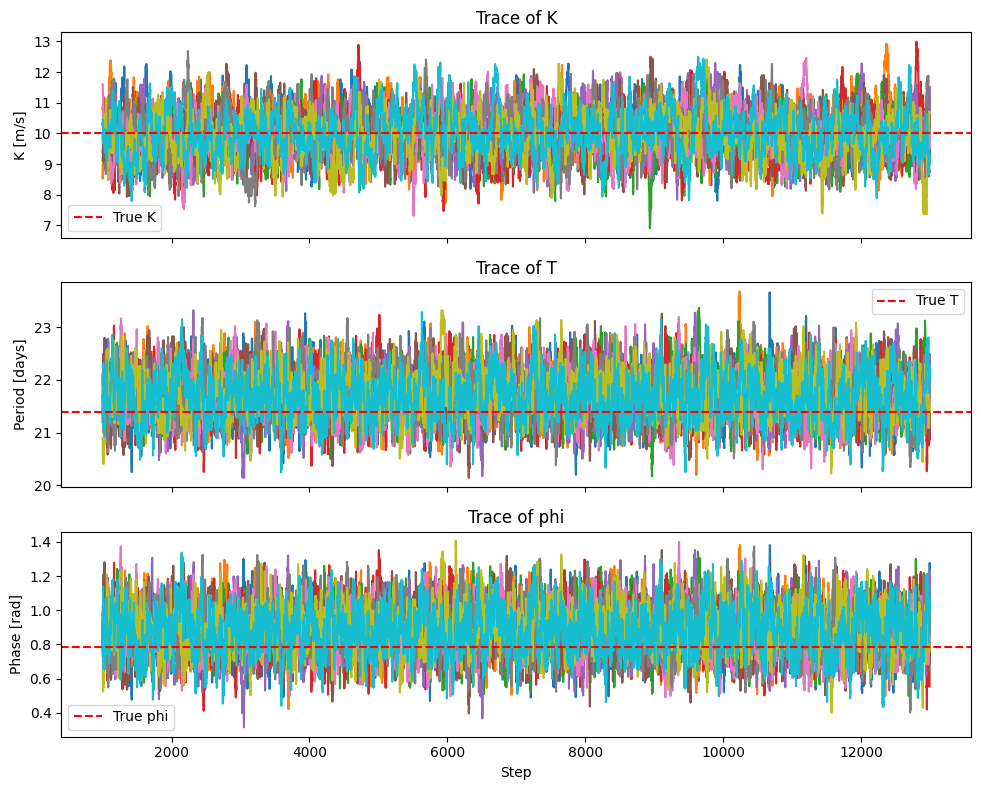
\includegraphics[width=\textwidth]{../scripts/2.5/figures/traces.png}
\caption{Trace plots of the Markov chains for each parameter. A total of 10 chains were run, each with 12,000 samples. The first 1,000 samples of each chain were discarded as burn-in.}
\label{fig:mcmc_trace}
\end{figure}

The trace plots of the chains are shown in \autoref{fig:mcmc_trace}. These are visualizations of the Markov chains for each parameter. The chains appear to be well-mixed and stationary, indicating that they have converged to the target distribution. Plotting the marginal posterior distributions of each parameter gives \autoref{fig:mcmc_posteriors}.

\begin{figure}[ht!]
\centering

\subfigure[$\mu = 10.02$ m/s $\quad \sigma = 0.73$ m/s]{%
    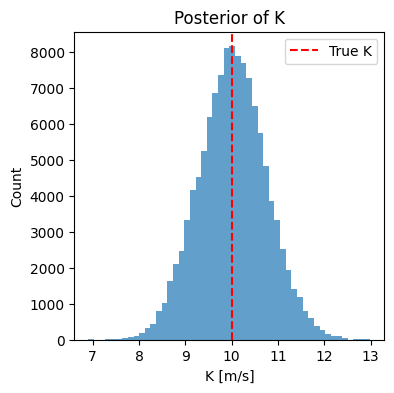
\includegraphics[width=0.32\textwidth]{../scripts/2.5/figures/k-posterior.png}%
    \label{fig:k_mcmc_posterior}%
}
\hfill
\subfigure[$\mu = 21.71$ days $\quad \sigma = 0.43$ days]{%
    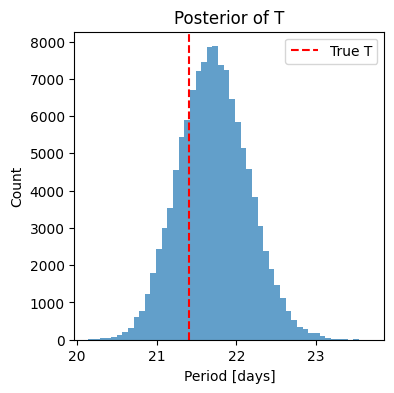
\includegraphics[width=0.32\textwidth]{../scripts/2.5/figures/t-posterior.png}%
    \label{fig:t_mcmc_posterior}%
}
\hfill
\subfigure[$\mu = 0.89$ rad $\quad \sigma = 0.13$ rad]{%
    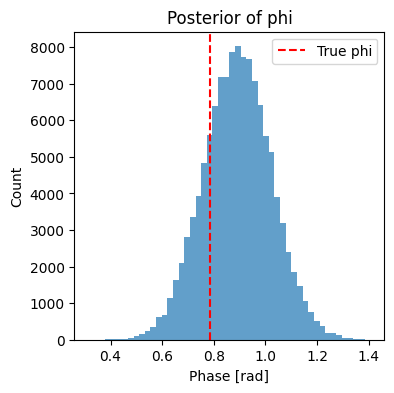
\includegraphics[width=0.32\textwidth]{../scripts/2.5/figures/phi-posterior.png}%
    \label{fig:phi_mcmc_posterior}%
}
\caption{The histograms of the draws from the posterior distributions of the parameters $K$, $T$, and $\phi$ given the data in \autoref{fig:rv_data}.}
\label{fig:mcmc_posteriors}
\end{figure}

Comparing these posteriors to the ones obtained using the brute-force method, we can see that they are very similar. \autoref{tab:comparison} summarizes the comparison between the true parameter values, the estimates from the brute-force method (\autoref{fig:bf_posteriors}), and the estimates from the MCMC method (\autoref{fig:mcmc_posteriors}). The two algorithms are compared using the mean and standard deviation of each posterior distribution, as well as the Z-score of the true value from the mean of each posterior distribution. The Z-score is a measure of how many standard deviations a value is from the mean, and is calculated as:
\begin{equation}
  Z = \frac{X - \mu}{\sigma},
\end{equation}
where $X$ is the value being compared, $\mu$ is the mean of the distribution, and $\sigma$ is the standard deviation of the distribution. A Z-score of 0 indicates that the value is equal to the mean, while a Z-score of 1 indicates that the value is one standard deviation above the mean. A Z-score of -1 indicates that the value is one standard deviation below the mean. A Z-score within the range of -2 to 2 is generally considered to be acceptable, as it indicates that the value is within two standard deviations of the mean.

\begin{deluxetable}{llllll}
  \tablewidth{0pt}
  \tablenum{2}
  \tablehead{
    \colhead{Parameter} & \colhead{True} & \colhead{Brute-Force} & \colhead{Brute-Force Z-score} & \colhead{MCMC}  & \colhead{MCMC Z-score}
  }
  \startdata
    $K$ (m/s) & $10.00$ & $9.99 \pm 0.73$ & -0.01 & $10.02 \pm 0.73$ & 0.03 \\
    $T$ (days) & $21.4$ & $21.72 \pm 0.44$ & 0.68 & $21.71 \pm 0.43$ & 0.66 \\
    $\phi$ (rad) & $0.25\pi$ & $0.89 \pm 0.13$ & 0.77 & $0.89 \pm 0.13$ & 0.77 \\
  \enddata
  \caption{Comparison of the true parameter values, the estimates from the brute-force method, and the estimates from the MCMC method.}
  \label{tab:comparison}
\end{deluxetable}

From \autoref{tab:comparison}, we can see that both methods give very similar results. The Z-scores of the true values from the means of each posterior distribution are all within 1, indicating that both methods were successful in estimating the parameters. The MCMC method, however, was far more computationally efficient. As shown in the code in \autoref{appx:A}, the brute-force method had to evaluate the posterior at $100^3 = 1,000,000$ points in the parameter space. The MCMC method, given in \autoref{appx:B}, only had to evaluate the posterior at $10 \times (12,000 - 1,000) = 110,000$ points, a reduction of nearly an order of magnitude, to provide virtually the same results.

Generalizing this to higher-dimensional parameter spaces, the computational savings of MCMC become even more apparent. In a hypothetical 10-dimensional parameter space with 100 possible values for each parameter, the brute-force method would have to evaluate the posterior at $100^{10} = 10^{20}$ points, which is infeasible. The MCMC method, on the other hand, would still only have to evaluate the posterior at $N$ points, where $N$ is the number of samples drawn, which is feasible for even high-dimensional parameter spaces.

\section{Case Studies}
\label{sec:CaseStudies}

\appendix
\section[Appendix A]{Radial Velocity Brute-Force Approach}
\label{appx:A}

\lstinputlisting[style=pythonstyle]{../scripts/2.2/brute-force-ex.py}

\section[Appendix B]{Radial Velocity MCMC Approach}
\label{appx:B}

\lstinputlisting[style=pythonstyle]{../scripts/2.5/mcmc-ex.py}

\bibliography{references}

\end{document}
